\documentclass[10pt]{article}
\usepackage{url}
\usepackage{color,graphicx}
\usepackage{amssymb,amsmath,amsthm,subfigure}
\usepackage[numbers]{natbib}
\usepackage{algorithm2e}
%\usepackage{almostfull}

%%% Environment for notation and a symbol command to go along with it.
%%% The argument should be the widest symbol which is expected if 
%%% \sym will be used to make the list.
%%%
\newenvironment{notation}[1]{%
\begin{list}{}{\small
\settowidth{\labelwidth}{{#1}\quad}%
\setlength{\itemsep}{1.5pt plus 0.5pt minus 0.2pt}%
\setlength{\parsep}{0ex}%
\setlength{\rightmargin}{0em}%
\setlength{\leftmargin}{\labelwidth}%
\addtolength{\leftmargin}{\labelsep}%
\addtolength{\leftmargin}{1em}}}{\end{list}}

\newcommand{\sym}[1]{\item[${#1}$\hfill{}]}

\newcommand{\bx}{\mathbf{x}}
\newcommand{\bu}{\mathbf{u}}
\newcommand{\tx}{\tilde{x}}
\newcommand{\norm}[1]{\vert #1 \vert}
\newcommand{\set}[1]{\left\lbrace #1 \right\rbrace}
%\newcommand{\SetAlgoLined}{}

\newcommand{\I}{\mathcal{I}}
\newcommand{\BO}{\textrm{BO}}
\newcommand{\IP}{\textrm{Ip}}
\newcommand{\UP}{\textrm{Up}}
\newcommand{\DN}{\textrm{Dn}}
\newcommand{\Inv}{\textrm{Iv}}
\newcommand{\Dem}{\textrm{Dm}}
\newcommand{\ulambda}{\underline{\lambda}}
\newcommand{\olambda}{\overline{\lambda}}
\newcommand{\eig}{\text{eig}}
\newcommand{\diag}{\text{diag}}

\newtheorem{assumption}{Assumption}
\newtheorem{theorem}[assumption]{Theorem}
\theoremstyle{definition}
\newtheorem{algo}[assumption]{Algorithm}
\newtheorem{definition}[assumption]{Definition}
\newtheorem{proposition}[assumption]{Proposition}
\newtheorem{remark}[assumption]{Remark}

\title{Cooperative  model predictive control: Current status and  limitations }
\author{Kaushik Subramanian \thanks{Department of Chemical and Biological
     Engineering, University of Wisconsin-Madison, U.S.A.}  \and James
  B. Rawlings\footnotemark[1] \thanks{Corresponding author: rawlings@engr.wisc.edu}}  
\begin{document}
\maketitle
\section{Introduction}
\label{sec:introduction}
Chemical plants are composed highly interconnected subsystems that
exchange material, energy and information with one another. Plant-wide
control strategies must take into account these interactions. Over the
past two decades, model predictive control has emerged as one of the
most commonly used control strategies in the process industry. 
In centralized model predictive control, the whole plant is considered
as a single system and a monolithic controller is designed. Although
offering good performance, the centralized controller can be hard to
implement and maintain. In decentralized control, the plant is
decomposed into many weakly interacting subsystems and the subsystems
are controlled independently \citep{sandell:varaiya:athans:safonov:1978}. It has been shown that decentralized
control can make the plant unstable \citep{cui:jacobsen:2002}. The middle ground is distributed
control, in which we seek to coordinate multiple controllers \citep{scattolini:2009}. A lot of
research focus has been dedicated to distributed control strategies
over the past decade.

In \citet{stewart:venkat:rawlings:wright:pannocchia:2010}, we proposed cooperative MPC, an architecture to coordinate
multiple controllers that had guaranteed closed-loop properties with
the additional feature that there was no coordinating layer or
coordinator. However, in that method, the assumptions on the types of model
allowed in each subsystem restricted the kinds of plants that we
control using cooperative MPC. Motivated by recent results in
nonlinear cooperative MPC \citet{stewart:wright:rawlings:2011}, we proposed a cooperative MPC controller
that could be used for any linear stabilizable plant and demonstrated
it on a supply chain example \citep{subramanian:rawlings:maravelias:2012}. 

In this paper, (i) we summarize the methods for cooperative MPC for linear
systems and discuss the advantages and disadvantages of each method
and (ii) propose an robust cooperative MPC algorithm based on
tube-based robust MPC \citep[Chapter 3]{rawlings:mayne:2009}.

In Section \ref{sec:suboptimal}, we briefly overview suboptimal MPC
theory which is the base upon which cooperative MPC is built. We then describe two flavors of cooperative MPC:
(i) Using Kalman decomposition of the state space (\ref{sec:substate})
and (ii) Using a relaxation of the terminal region
(\ref{sec:relaxation}). In Section \ref{sec:tube}, we present the
tube-based cooperative MPC algorithm for robust cooperative
control. Finally, in Section \ref{sec:related}, we briefly outline
related work in cooperative MPC before concluding in Section
\ref{sec:conclusions}.

\section{Suboptimal MPC}
\label{sec:suboptimal}
Model predictive control is a rolling horizon optimization
based control algorithm. In MPC, at each sampling time, an on-line
optimization problem is solved to find the control actions over a
finite prediction horizon. Only the first of these control actions (that corresponds to the control
action at the current sampling instance) is injected to the plant and
the whole process is repeated again at the next sampling time. Thus,
to study the controller, we need to focus, not only on the
optimization problem solved at each sampling time, but also on the
dynamics of the system with the injected move. Lyapunov theory is an
convenient tool to study the stability and convergence properties of
dynamic systems and MPC design procedures using Lyapunov theory has
been widely studied. In Optimal MPC \citep[Chapter
  2]{rawlings:mayne:2009}, the on-line optimization problem needs to
be solved to optimality to ensure closed-loop properties like
stability and asymptotic convergence. In Suboptimal MPC
\citep{pannocchia:rawlings:wright:2011,scokaert:mayne:rawlings:1999},
the same closed-loop properties can be ensured without requiring
the on-line problems to be solved to optimality. In the following
section, we briefly review the design procedure for ensuring
closed-loop stability in suboptimal MPC and introduce the parallel
optimization algorithm that we use in cooperative MPC so that
cooperative MPC is a special case of suboptimal MPC.
 
\subsection{Preliminaries}
Consider a system comprising of $M$ subsystems described by the
following linear dynamics: 

\begin{equation}
\label{eq:model}
x^+ = Ax + \sum_{i=1}^{M} B_i u_i
\end{equation}
The states of the system are described by $x$, while $x^+$ denotes the
state at the next sampling instance. The input is given by $u =
(u_1,u_2,\ldots,u_M)$. The input $u_i$ is manipulated by subsystem-$i$.

The states are constrained to lie in the set $\mathbb{X}$ while the
inputs are constrained to lie in the set $\mathbb{U}$.

The MPC objective function is defined as:
\begin{equation}
\label{eq:VN0}
V_N(x,\bu) = \sum_{j=0}^{N-1}\ell(x(j),u(j)) + V_f(x(N))
\end{equation}
in which $N$ is the control horizon, $\bu = (u(0),u(1),\ldots,u(N-1))$
is the input vector and $x(j)$ is the short-hand notation for the
state evolution under the input $\bu$. That is,
 \[x(j) = \phi(j;x,\bu)=  A^{j-1}x +\sum_{l=0}^{j-1} A^lBu(j-1-l)\]
in which $B = \begin{bmatrix}B_1&B_2&\ldots&B_M\end{bmatrix}$.

The cost function $V_N(x,\bu)$ consists of the stage cost
$\ell(x(j),u(j)$ and the terminal cost $V_f(x(N))$. The costs are
chosen to be positive definite quadratic cost:
\begin{equation}
\label{eq:costs}
\ell(x,u) = x'Qx + u'Ru \qquad V_f(x) = x'Px 
\end{equation}
in which $R>0, P>0,Q > 0$.

We define the terminal region as the set $\mathbb{X}_f$.

The on-line optimization problem that is solved is:

\begin{xalignat}{2}
\mathbb{P}_N(x): & \min_{\bu}V_N(x,\bu) & \nonumber \\
& \text{s.t~} x(j+1) = Ax(j) + Bu(j)&  \forall j \in 0,1,\ldots,N-1\nonumber\\
& x(j) \in \mathbb{X},&   \forall j \in 0,1,\ldots,N-1 \nonumber \\
& u(j) \in \mathbb{U}, &\forall j \in 0,1,\ldots,N-1  \label{eq:PNx}\\
& x(0) = x \nonumber \\
& x(N) \in \mathbb{X}_f \nonumber
\end{xalignat}


We define the set $\mathbb{Z}$ as the feasible region of the problem
$\mathbb{P}_N(x)$. That is,
\[ \mathbb{Z} = \set{(x,\bu) \mid \phi(j;x,\bu) \in \mathbb{X},
  \phi(N;x,\bu) \in \mathbb{X}_f, \bu \in \mathbb{U}^N}
\]

The projection of the feasible space onto $x$ is the set of feasible
inputs for a given initial state $x$. This set is denoted by
$\mathcal{U}_N(x)$ and is given by:

\[ \mathcal{U}_N(x) = \set{\mathbb{\bu} \mid (x,\bu) \in \mathbb{Z}}
\]

\subsection{Closed-loop properties of suboptimal MPC}
The following assumptions are made on the system:
\begin{assumption}
\label{ass:stab}
The centralized system $(A,B)$
is stabilizable.  
\end{assumption}

\begin{assumption}
\label{ass:psd}
The cost functions $\ell(x,u)$ and $V_f(x)$ are positive definite.
\end{assumption}
\begin{assumption}
\label{ass:bsa}
The set $\mathbb{X}_f$ and the  costs $\ell(x,u),V_f(x)$ are chosen
such that there exists a controller $u = \kappa_f(x)$ that satisfies:
\begin{xalignat}{1}
\label{eq:bsa}
V_f(Ax+B\kappa_f(x)) -V_f(x) \leq -\ell(x,\kappa_f(x)) &\qquad \forall x
\in \mathbb{X}_f \\
Ax + B\kappa_f(x) \in \mathbb{X}_f, \kappa_f(x) \in \mathbb{U}& \qquad
\forall x \in \mathbb{X}_f
\end{xalignat}
\end{assumption} 

\begin{assumption}
\label{ass:closed}
The set $\mathbb{U}$ is closed and compact and contains the origin in
its interior. The set $\mathbb{X}$ is closed and contains the origin
in its interior. The set $\mathbb{X}_f$ is closed and compact and
contains the origin in its interior.
\end{assumption}

\begin{remark}
The choice of quadratic stage and terminal costs with $Q > 0, P >0,
R>0$ automatically satisfies Assumption \ref{ass:psd}.
\end{remark} 

\begin{remark}
From Assumption \ref{ass:stab}, we know that there exists a linear
feedback $K$ such that $(A+BK)$ is stable. In other words, the
closed-loop $x^+ = (A+BK)x$ is stable. We choose such a $K$ as the
terminal controller $\kappa_f(x)$. The terminal penalty $V_f(x) =
x'Px$ is chosen as 
the solution to the Lyapunov equation (which exists as a consequence
of Assumption \ref{ass:psd}):
\[ (A+BK)'P(A+BK) + (Q+K'RK) = P \]

For the pair $(P,K)$, we can define the control invariant region in
the state-space in which $u=Kx$ does not activate any constraints as:
\[ \mathbb{X}_f := \set{x \mid x^+= (A+BK)x \in \mathbb{X}_f \subseteq
  \mathbb{X}, Kx \in \mathbb{U}}
\]

For linear systems, such sets can be easily constructed. See
\citet{gilbert:tan:1991} for an algorithm. 
\end{remark}

As the name suggests, in suboptimal MPC, we wish to inject {\emph{some}} feasible input
to the plant. In order to ensure that despite injecting suboptimal
inputs to the plant, we maintain the desirable closed-loop properties,
we define the warm start and the successor input set as follows. We
denote $\kappa_s(x)$ as the first input in the suboptimal input
sequence.

\begin{definition}[Warm Start]
\label{def:warmstart}
Let $(x,\bu)$ be a state-input vector pair such that $\bu$ is feasible
for $\mathbb{P}_N(x)$.  Then the warm start for the successor initial state
$x^+ = Ax+B\kappa_s(x)$ is defined as:
\begin{equation*}
%\label{eq:warmstart}
\tilde{\bu} = \left (\bu(1;x),\bu(2;x),\ldots,\bu(N;x),u_+\right)
\end{equation*}
in which  $u_+ = \kappa_f(\phi(N;x,\bu))$.
\end{definition}
\begin{definition}[Successor input set]
\label{def:G}
Consider $(x,\bu)$ such that $\bu$ is feasible for
$\mathbb{P}_N(x)$. For the  successor state 
$x^+ = Ax+B\kappa_s(x)$, we define the set $G(x,\bu)$
\begin{multline*}
G(x,\bu) = \lbrace \bu^+ \mid \bu^+ \in
\mathcal{U}(x^+), V(x^+,\bu^+)\leq V(x,\tilde{\bu}), \\
V(x^+,\bu^+) \leq V_f(x^+) \text{~if~} x\in r\mathbb{B} \rbrace
\end{multline*}
in which $\tilde{\bu}$ is the warm start given by Definition 
\ref{def:warmstart} and $r\mathbb{B}$ is a ball of radius $r>0$. We
choose $r$ sufficiently small such that  
$r\mathbb{B}$ is a subset of the terminal region. We can show that
this constraint is equivalent to  $\bu_i \leq d_i \norm{x}, x \in
r\mathbb{B},d_i >0, i \in 1,2,\ldots,M$ \citep{subramanian:rawlings:maravelias:2012}.  
\end{definition}

\begin{theorem}
\label{thm:suboptimal}
Let Assumptions \ref{ass:stab} and \ref{ass:closed}
hold. Choose optimization problem $\mathbb{P}_N(x)$ and the appropriate terminal
regions. For any $x$ for which  $\mathcal{U}(x)$  is not empty, choose
$\bu \in \mathcal{U}(x)$. Then, the origin of the closed-loop system 
\begin{align*}
x^+ &= Ax+ B\kappa_s(x) \\
\bu^+ &\in G(x,\bu)
\end{align*}
is asymptotically stable on (arbitrarily large) compact  subsets of
the feasible region $\mathcal{X}_N :=\set{x\mid \exists u \in
  \mathbf{U}^N, \text{~s.t~} \mathcal{U}_N(x) \neq \varnothing}$. 
\end{theorem}

The proof of Theorem \ref{thm:suboptimal} is presented in
\citep{pannocchia:rawlings:wright:2011}.

Observe that for the nominal system, the warm start is a member of the
set $G(x,\bu)$.  Therefore, if we have a feasible $(x,\bu)$ pair, we
can construct an asymptotically stable closed loop without any
optimization.  However, if we wish to improve performance by
optimization, we need the optimization algorithm to have the
following properties: 
\begin{definition}
\label{thm:propO}
The optimization algorithm applied to $\mathbb{P}_N(x)$ has the following properties:
\begin{enumerate}
\item It is an iterative algorithm starting from a feasible point $(x,\tilde{\bu})$.
\item Every iteration $\bu$ decreases the objective function. 
\item Every iteration is feasible.
\end{enumerate}
\end{definition}
Properties (2) and (3) ensure that {\em{any intermediate iterate}}
generated by the algorithm  belongs to the set
$G(x,\bu)$. Hence, we need not  wait for the optimizations to converge
and can inject the suboptimal input from any iterate to the plant
without compromising the closed-loop properties.


\begin{remark} The properties of the optimizer given by Definition
\ref{thm:propO} means that not all optimization algorithms is suitable
for suboptimal MPC. For example, parallel solvers that use a dual
relaxation achieve feasibility only at convergence and hence
the intermediate iterates are infeasible. Such optimizers are not
suitable for suboptimal MPC.
\end{remark}

In the following section, we present the
Jacobi parallel optimization algorithm tailored for cooperative MPC.

\subsection{Cooperative MPC}
In Cooperative MPC, we assume that each subsystem knows (i) the
overall system model \eqref{eq:model} and (ii) the overall system
objective function \eqref{eq:VN0}. With the knowledge of the system-wide model and objective
function, each subsystem then solves the centralized
MPC problem \eqref{eq:PNx}. Each subsystem shares (i) its current
decision variable $\bu_i$ with all the other subsystems, (ii)
optimizes the centralized problem over its decision variables having
fixed the decision variables of the other sub-systems at the shared
value, and (iii) makes the control move without requiring any
coordinating layer.

For subsystem $i$, we denote all the other subsystems as
$-i$. The following is the optimization problem for subsystem
$i$ in which $\mathbf{\bu}_{-i} =
(\bu_1,\bu_2,\ldots,\bu_{i-1},\bu_{i+1},\ldots,\bu_M)$.

\begin{xalignat}{2}
\mathbb{P}^{i}_N(x,\mathbf{v}_{-i}): & \min_{\bu_i}V_N(x,\bu)& \nonumber \\
& \text{s.t~} x(j+1) = Ax(j) + Bu(j) & \forall j \in 0,1,\ldots,N-1\nonumber\\
& x(j) \in \mathbb{X}& \nonumber \\
& u(j) \in \mathbb{U}&\label{eq:PNxu} \\
& u_{-i}(j) = v_{-i}(j),  \qquad & \forall j \in 0,1,\ldots,N-1 \nonumber\\
& x(0) = x& \nonumber \\
& x(N) \in \mathbb{X}_f& \nonumber
\end{xalignat}


\begin{algo}[Cooperative MPC] \mbox{ }
\label{alg:coop}

\begin{algorithm}[H]
 \KwData{Starting state $x(0)$, initial guess
   $(\tilde{\bu}_1(0),\tilde{\bu}_2(0),\ldots,\tilde{\bu}_M(0)) \in \mathcal{U}_N(x(0))$,
   $\bar{p} \geq 1$ and $\omega_i \in (0,1)$ such that
   $\sum_{i=0}^{M}\omega_i = 1$}
 \KwResult{Asymptotically stable closed loop}
 set $k \leftarrow 0$ \\
 \While {$k \geq 0$}{
   Set $p \leftarrow 0$, $x \leftarrow x(k)$\\
   Set $\bu_i^{(p)} \leftarrow \tilde{\bu}_i(k)$ for $i = 1,2,\ldots,M$\\
   Broadcast current subsystem inputs $\tilde{\bu}_i(k)$ to other
   subsystems \\
   \While {$p < \bar{p}$}{
       Solve $\mathbb{P}_N^{i}(x,\bu_{-i})$ to obtain
       $\bu_i^0$ for i in $1,2,\ldots,M$ \\
       Set $\bu_i^{(p+1)} \leftarrow \omega_i \bu_i^{(p)} +
       (1-\omega_i) \bu_i^0$ for i in $1,2,\ldots,M$ \\
   }
  Set $\bu \leftarrow (\bu_1^{(p)},\bu_2^{(p)},\ldots,\bu_M^{(p)})$ and find $x(k+N) \leftarrow
  \phi(N;x(k),\bu)$\\
  Obtain $u_+ = (u_{1+},u_{2+},\ldots,u_{M+}) \leftarrow \kappa_f(x(k+N))$\\
  Obtain warm start $\tilde{\bu}_i(k+1) =
    (\bu_i^{(p)}(1),\bu_i^{(p)}(2),\ldots,u_{i+})$ for $i = 1,2,\ldots,M$.\\
   Set input as $u(k) =
  (\bu_1^{(p)}(0),\bu_2^{(p)}(0),\ldots,\bu_M^{(p)}(0))$\\
  Evolve state from $x(k)$ to $x(k+1)$ under input $u(k)$\\
 }
\end{algorithm}
\end{algo}

The convergence properties of cooperative MPC described in Algorithm
\ref{alg:coop} is based on (i)Design of the terminal region so that warm start is a member of
  $G(x,\bu)$. Therefore, we can use Theorem \ref{thm:suboptimal} to
  prove closed-loop properties, and (ii) Control performance improvement by reducing the objective
 because of Jordan type parallel optimization algorithm in the inner
 loop of the cooperative MPC algorithm \citep[Section
3.3.5]{bertsekas:tsitsiklis:1989}. Therefore, we can ensure that each
iteration of cooperative MPC generates a feasible input move that
improves the control objective.  

Optimization algorithm in the inner loop of Algorithm \ref{alg:coop} satisfies requirements in Definition\ref{thm:propO}
for convex optimization problems. In addition, if there are no coupled
constraints between the subsystems, then we can ensure that that the
iterates generated by the algorithm converge to the centralized
optimal solution. 

The on-line optimization problem in MPC for linear systems given by
$\mathbb{P}_N(x)$ \eqref{eq:PNx} is a convex optimization problem with
coupled constraints between subsystems. The coupled constraints are
(i) the state constraints, (ii) the input constraints and, (iii) the
terminal constraints.

Closed-loop stability and asymptotic stability  guarantees for
cooperative MPC are ensured by Theorem \ref{thm:suboptimal} if we use
Algorithm \ref{alg:coop} as the cooperative MPC parallel
optimization algorithm. However,
we cannot guarantee performance, that is, we cannot conclude that if
$\bar{p} \rightarrow \infty$, then the solution obtained by
cooperative MPC is the centralized optimal solution. To do so, we have
to remove the coupled constraints in the on-line MPC problem. Hence,
we make the following assumptions for cooperative MPC:

\begin{assumption}
\label{ass:noX}
There are no state constraints. State constraints are enforced as
soft-penalties by tuning the $Q$ matrix in the stage cost.
\end{assumption}

\begin{assumption}
\label{ass:uncoupledU}
The input constraint space is uncoupled. That is, the input constraint
set $\mathbb{U}$ is the Cartesian product of the input constraint sets
of each subsystem. 
\[ \mathbb{U} = \mathbb{U}_1 \times \mathbb{U}_2 \times \ldots \times
\mathbb{U}_M
\]
\end{assumption}

The only remaining coupled constraint is the terminal region
constraint which needs to be enforced to guarantee stability and
asymptotic convergence. In the next two sections, we briefly review
two techniques to ``uncouple'' the terminal region constraint.

\subsubsection{Sub-states}
\label{sec:substate}
We consider a non-minimal realization of the system \eqref{eq:model}
such that ``sub-state'' $x_{il}$ in subsystem $i$ is only influenced
by input $l$. That is:
\begin{equation}
\label{eq:substate}
 \tilde{x}_{il}^+  = \tilde{A}_{il} x_{il}  + \tilde{B}_{il} u_l
\end{equation}


The states that are influenced only by input $i$ are  given by $\tilde{x}_i =
(\tilde{x}_{1i},\tilde{x}_{2i},\ldots,\tilde{x}_{Mi})$. The outputs are functions of the
state, that is,

\begin{equation}
\label{eq:Cx}
y=  C\begin{bmatrix}\tilde{x}_1\\\tilde{x}_2\\\vdots\\\tilde{x}_M\end{bmatrix}
\end{equation}

In this paper, we assume that the output $y$'s are the centralized
states $x$ in \eqref{eq:model}. 

The terminal region is now modified as :
\begin{equation}
\label{eq:zero_terminal}
\mathbb{X}_f = \set {\tilde{x}_{il} = 0\qquad  \forall i \in 1,2,\ldots,M;
\forall l \in 1,2,\ldots,M }
\end{equation}

The {\em{centralized}} optimization problem now becomes:

\begin{xalignat}{2}
\mathbb{P}_N(x): & \min_{\bu}V_N(x,\bu)& \nonumber \\
& \text{s.t~} \tilde{x}_{li}(j+1) = \tilde{A}\tilde{x}_{li}(j) +
\tilde{B}_{li}\tilde{u}_i(j) & \forall l \in 1,2,\ldots,M\nonumber\\
&\qquad & \forall i \in 1,2,\ldots,M,\forall j \in 0,1,\ldots,N-1 \nonumber\\
& u_i(j) \in \mathbb{U}_i& \forall i \in 1,2,\ldots,M, \forall j \in
0,1,\ldots,N-1 \label{eq:PNx_substate_centralized}\\
& x(0) = x& \nonumber \\
& x_{li}(N) = 0 & \forall \set{l,i} \in 1,2,\ldots,M  \nonumber
\end{xalignat}

Since each substate $\tilde{x}_{il}$ dynamics is influenced only by a
single input \eqref{eq:substate}, the terminal constraints
\eqref{eq:zero_terminal} are uncoupled. 

Therefore, each subsystem $i$ solves the following optimization
problem:

\begin{xalignat}{2}
\mathbb{P}^{i}_N(x,\mathbf{v}_{-i}): & \min_{\bu_i}V_N(x,\bu)& \nonumber \\
& \text{s.t~} \tilde{x}_{li}(j+1) = \tilde{A}\tilde{x}_{li}(j) +
\tilde{B}_{li}\tilde{u}_i(j) & \forall l \in 1,2,\ldots,M\nonumber\\
& \qquad&  \forall j \in 0,1,\ldots,N-1 \nonumber\\
& u_i(j) \in \mathbb{U}_i&\forall j \in 0,1,\ldots,N-1 \label{eq:PNxu_substate} \\
& x(0) = x& \nonumber \\
& x_{li}(N) = 0 & \forall l \in 1,2,\ldots,M  \nonumber
\end{xalignat}

Note that we have not written the constraints for the state
dynamics and terminal constraints for the states that are not
influenced by input $i$. If Assumption \ref{ass:stab_substate} is
satisfied, then  Algorithm \ref{alg:coop} can be used to
stabilize the plant {\em{with guaranteed performance}} to the
centralized solution to problem \eqref{eq:PNx_substate_centralized} as
there are no coupled constraints in problem
\eqref{eq:PNx_substate_centralized} \citep{stewart:venkat:rawlings:wright:pannocchia:2010}
Assumption \ref{ass:stab_substate} ensures that (i) the input $\bu_i$ can be used to
zero all the states that $u_i$ influences, (ii) all the outputs can be
reconstructed from the substates.

\begin{assumption}[Subsystem stabilizability]\mbox{ }
\label{ass:stab_substate}
\begin{itemize}
\item The system $(\underline{A}_i,\underline{B}_i)$ is stabilizable, in
which  $\underline{A}_i,\underline{B}_i$ are defined as:
\begin{align*}
\underline{A}_i &= \text{diag}(\tilde{A}_{1i},\tilde{A}_{2i},\ldots,
\tilde{A}_{li}, \ldots, \tilde{A}_{Mi})\\
\underline{B}_i
&= \begin{bmatrix}\tilde{B}_{1i}\\\tilde{B}_{2i}\\\vdots\\\tilde{B}_{li}\\\vdots\\\tilde{B}_{Mi}\end{bmatrix}
\end{align*}
\item The system $(A,C)$ is detectable, in which $A$ is given by
\[ A = \diag(\underline{A}_1,\underline{A}_2,\ldots,\underline{A}_m)
\]
and $C$ is the matrix from \eqref{eq:Cx}.
\end{itemize}
\end{assumption}

We now discuss the features of the aforementioned decomposition:

\paragraph{Applicability.} The decomposition into the substate models
\eqref{eq:substate} can be obtained from the Kalman decomposition of
the original input/output $y_i,u_i$ model
\citep[p.270]{antsaklis:michel:1997}.

The drawback however, is that not all centralized stabilizable models
have a corresponding subsstate non-minimal realization that satisfies
Assumption \ref{ass:stab_substate}. One such example is the system of
integrators (like supply chain models) that was discussed in
\citet{subramanian:rawlings:maravelias:2012}.

\paragraph{Convergence.} The decomposition ensures that if the inner
optimization loop in Algorithm \ref{alg:coop} is allowed to converge,
then the solution is the centralized solution to the optimization
problem \eqref{eq:PNx_substate_centralized}. However, we cannot
guarantee convergence to the problem \eqref{eq:PNx}. The main
advantage of problem \eqref{eq:PNx} is that it admits a larger region
of attraction because it has a (possibly) larger terminal region.

\paragraph{Initialization.} The optimization lop in Algorithm
\ref{alg:coop} requires an feasible starting point. The feasible
starting point is ensured by the warm start. The warm start
is feasible because we assume that the actual plant state at the next
sampling time is equal to the model prediction for the next state. In
many cases, when there are plant-model mismatches or unmodeled
disturbances affecting the system, this assumption that the plant
state is equal to the predicted state might break-down. In such cases,
the warm start becomes infeasible and we need an distributed
initialization routine.

In the substate decomposition of the model, the warm start is
infeasible if $\tilde{x}_{il}(N;x,\bu) \neq 0$ for some
$i,l$. However, since $\tilde{x}_{il}(N;x,\bu)$ only depends on the
input sequence from a single subsystem $\bu_l$, the re-initialization
routine is also decoupled. In other words, the initialization routine
that each subsystem has to solve at time $j$ if the warm-start is
infeasible is select a new input sequence $\mathbf{v}_i$ from the
following set:

\[ \mathcal{U}_i(x) \in \set{ \mathbf{v}_i \mid \mathbf{v}_i \in
  \mathbb{U}_i^N; \tilde{x}_{li}(N;x,\mathbf{v}_i) = 0 \forall \set{l,i} \in
  1,2,\ldots,M}
\]

\subsubsection{Relaxing the terminal region}
\label{sec:relaxation}
In this section, we work with the (minimal) centralized model
\eqref{eq:model}. The idea here is to develop an optimization problem
without terminal constraints such that every every iterate generated
in the inner optimization loop of Algorithm \ref{alg:coop} lies inside
a terminal region that satisfies Assumption \ref{ass:bsa}. To do so,
we modify (i) the terminal region (ii) the cost function and (iii) the
feasible set as follows:

The terminal region is chosen as a sublevel set of the terminal
cost. That is,

\begin{equation}
\label{eq:Xfa}
\mathbb{X}_f := \set{x \mid V_f(x) \leq a, a > 0}
\end{equation}

For linear systems, we could use $P$, the solution to the Lyapunov
equation as $V_f(x)$ and choose $a$ such that all the requirements in
Assumption \ref{ass:bsa} are satisfied.

The cost function is modified so that the terminal penalty is
magnified. That is,

\begin{equation}
\label{eq:VNbeta}
V_N(x,\bu) = \sum_{j=0}^{N-1} \ell(x(i),u(i)) + \beta V_f(x(N))
\end{equation}
in which $\beta \geq 1$.

Finally, the feasible set is modified as follows:
\begin{equation}
\label{eq:ZNbeta}
\mathbb{Z} = \set{ (x,\bu) \mid V_N(x,\bu) \leq \bar{V}, u \in
  \mathbb{U}^N}
\end{equation}
in which $\bar{V} \geq 0$  can be chosen arbitrarily large.

In Proposition \ref{prop:betabar}, we show how the parameter $\beta$
can be chosen so that if $(x,\bu) \in \mathbb{Z}$, then
$x(N;x,\bu) \in \mathbb{X}_f$. 

\begin{proposition}
\label{prop:betabar}
Let the cost function be given by $V_N(x,\bu)$ \eqref{eq:VNbeta}. For  $\bar{V}
\geq a $, define $\bar{\beta} := \bar{V}/a$. Then, for any $\beta \geq
\bar{\beta}$ and $(x,\bu) \in \mathbb{Z}$ \eqref{eq:ZNbeta}, we have
that $\phi(N;x,\bu) \in \mathbb{X}_f$ in which $\mathbb{X}_f$ is given
by \eqref{eq:Xfa}. 
\end{proposition}
The proof is by contradiction and is presented in
\citet{subramanian:rawlings:maravelias:2012}. The centralized MPC
problem is therefore:
\begin{xalignat}{2}
\mathbb{P}_N(x): & \min_{\bu}V_N(x,\bu) &\nonumber \\
& \text{s.t~} x(j+1) = Ax(j) + Bu(j) &  \forall j \in 0,1,\ldots,N-1\nonumber\\
& u(j) \in \mathbb{U} & \forall j \in 0,1,\ldots,N-1  \label{eq:PNxbeta} \\
& x(0) = x & \nonumber
\end{xalignat}

in which $V_N(X,\bu)$ is given by \eqref{eq:VNbeta}. Notice that we do
not enforce any terminal constraints in problem \eqref{eq:PNxbeta}
because they are automatically satisfied by the choice of $\beta$  and
$\mathbb{Z}$. That is, we restrict the feasible states to lie in:
\[ \mathcal{X} : \set{ x \mid \exists \bu \in \mathbb{U}^N \text{s.t~}
  (x,\bu) \in \mathbb{Z}}
\]
in which $\mathbb{Z}$ is given by \eqref{eq:ZNbeta}. 

Companion to problem \eqref{eq:PNxbeta}, we write the cooperative
MPC optimization problem for each subsystem as:
\begin{xalignat}{2}
\mathbb{P}^{i}_N(x,\mathbf{v}_{-i}): & \min_{\bu_i}V_N(x,\bu)& \nonumber \\
& \text{s.t~} x(j+1) = Ax(j) + Bu(j) &\forall j \in 0,1,\ldots,N-1\nonumber\\
& u_i(j) \in \mathbb{U}_i&\forall j \in 0,1,\ldots,N-1\label{eq:PNxubeta} \\
& u_{-i}(j) = v_{-i}(j),  \qquad \forall j \in 0,1,\ldots,N-1 \nonumber\\
& x(0) = x& \nonumber 
\end{xalignat}

Since the problem \eqref{eq:PNxbeta} has no coupled constraints, we
can ensure that the inner-loop of Algorithm \ref{alg:coop} converges
to the optimal solution of \eqref{eq:PNxbeta}. Note that in Algorithm
\ref{alg:coop}, the set $\mathcal{U}_N(x)$ now corresponds to:
\[ \mathcal{U}_N(x) = \set{\bu \mid (x,\bu) \in \mathbb{Z}
}
\]
in which $\mathbb{Z}$ is given by \eqref{eq:ZNbeta}.

We now discuss the features of the aforementioned relaxation:
\paragraph{Applicability.} The relaxation is applicable to any
stabilizable centralized system. 

\paragraph{Convergence.} As mentioned earlier, the relaxation ensures
that the inner optimization loop of Algorithm \ref{alg:coop} converges
to the optimal solution of \eqref{eq:PNxbeta}. 

As shown in
\citet{pannocchia:rawlings:wright:2011}, for a fixed $a$, as we
increase $\bar{V}$, the set $\mathbb{Z}$ approaches the following set:
\[\bar{\mathbb{Z}} =  \set{(x,\bu) \mid \exists \bu \in \mathbb{U}^N,
  \phi(N;x,\bu) \in \mathbb{X}_f}\]
Therefore, we could cover as much of the  feasible space  of the original
centralized problem \eqref{eq:PNx} by increasing $\bar{V}$, and
selecting $a$ so that the terminal region covers most of the polytopic
terminal set in the original centralized problem presented in the
previous section.

The main drawback of the
relaxation method is that the hessian of the objective could get
ill-conditioned due to the choice of $\bar{V}$ and $a$.

\paragraph{Initialization.} As mentioned in the previous section, the
warm start could become infeasible. From Proposition
\ref{prop:betabar}, it is clear that an infeasible warm start
indicates that $V_N(x,\tilde{\bu}) > \bar{V}$. However, note that
warm-start does not make the optimization problem \eqref{eq:PNxubeta}
infeasible. Since the inner loop optimizations decrease the objective
values at each iteration, there is an iteration $p'$ so that  $V_N(x,\bu^{(p)})
\leq \bar{V}$ for $p \geq p'$.  
After $p'$ iterations of the inner optimization loop, we would have 
ensured that the stability requirements are satisfied. The drawback is, unlike the regulation problem
with a feasible warm start, we cannot terminate the inner-loop
optimizations arbitrarily after any number of iterations. For small
infeasibilities, we can expect the algorithm to regain feasibility in
a few iterations, but we do not have a theoretical upper-bound on the
number of iterations, $p'$, required to regain feasibility.

\section{Robust cooperative MPC}
\label{sec:tube}
\subsection{Preliminaries}
We consider the system \eqref{eq:model} subject to bounded additive
disturbance as follows:
\begin{equation}
\label{eq:model_dist}
x^+ = Ax + \sum_{i=1}^{M} B_i u_i + w
\end{equation}
in which the inputs are assumed to lie in set $u_i \in \mathbb{U}_i$
as in the previous section. The assumptions on the disturbance are
stated in Assumption \ref{ass:W}

\begin{assumption}[Bounded disturbance]
\label{ass:W}
The additive disturbance $w$ lies in a compact set $\mathbb{W}$
containing the origin in its interior.
\end{assumption}

The nominal system, without the additive disturbance is denoted as
follows using $z,v$ for the nominal state and input variables.

\begin{equation}
\label{eq:model_nominal}
z^+ = Az + \sum_{i=1}^{M} B_i v_i
\end{equation}

At any time $k$, we can write the deviation between the actual state
and the nominal stats as $e(k) = x(k)-z(k)$. If the inputs to both the
nominal and actual system were the same, then the error dynamics can
be written as:

\begin{equation}
\label{eq:error_dynamics}
e^+ = Ax+Bu+w - Az+Bu = Ae + w
\end{equation}

Hence, given an initial $e(0)=0$, the error at time $k$ lies in the
following set:

\begin{equation}
\label{eq:error_set}
e(k) \in S(i) :=\sum_{j=0}^{k-1}A^j\mathbb{W} = \mathbb{W} \oplus A\mathbb{W}
\oplus \ldots \oplus A^{k-1}\mathbb{W}
\end{equation}
in which $A^j\mathbb{W}$ indicates set multiplication. That is,

\[A^j\mathbb{W} := \set{A^jw \mid \forall w \in \mathbb{W}}
\]

The symbol $\oplus$ indicates set addition. That is,
\[ \mathbb{W} \oplus A\mathbb{W} := \set{w_1+w_2 \mid w_1 \in
  \mathbb{W}, w_2 \in A\mathbb{W}}\]

For stable $A$, it can be shown that the set $S(\infty)$ exists and is
positive invariant for the system \eqref{eq:error_dynamics}
\citep{kolmanovsky:gilbert:1998}.


\subsection{Tube based MPC}

We now discuss tube based MPC, the basic idea for which is as follows: (i)
use MPC on the nominal system to find $v(k) = \kappa(z(k))$,  and (ii)
based on the error at time $k$, $e(k)$, find the input to the plant as $u(k) = v(k) + Ke(k)$

By design, we select a $K$ such that $A_K:=A+BK$ is Hurwitz. Such a choice
implies that the error dynamics in the closed-loop is:
\begin{equation}
\label{eq:error_CL}
e^+ = x^+-z^+=Ax+Bv+BK(x-z)+w-Az-Bv = A_Ke+w
\end{equation}

Now, since $A_K$ is stable, we can conclude that $S_K(\infty) =
\sum_{j=0}^{\infty}A_K^j\mathbb{W}$ exists and is positive invariant
for \eqref{eq:error_CL}.

The stability and convergence theorems are therefore based upon the
following observations:(i) the origin is asymptotically stable for the
nominal system $z^+= Az+B\kappa(z)$ by design. The MPC control law is
denoted by $\kappa(z)$, (ii) the error is designed to lie in the set
$S_K(\infty)$ by the   choice of $K$ and input $u = \kappa(z) +
K(x-z)$, and (iii) the actual state $x(k); k \rightarrow \infty$
therefore belongs to the set   $\set{0} \times S_K(\infty)$

In the presence of persistent disturbance, we ensure that the states
lie inside a bounded set that we can compute offline. The name tube
based MPC comes from the fact that at each time $k$, the state $x$
lies in a ``tube'' defined by $x(k) \in z(k)\oplus S_K(k)$. 

For the inputs $u = v+K(x-z)$ to remain feasible, we need to ensure
that $v$ satisfies the tighter constraints:
\begin{equation}
\mathbb{V}(k) := \mathbb{U} \ominus KS_K(k)
\end{equation}
The tighter set follows from the fact that $e = (x-z) \in
S_K(k)$. 

The nominal MPC problem is defined as:
\begin{align}
\tilde{\mathbb{P}}_N(z): & \min_{\bu}V_N(z,\mathbf{v}) \nonumber \\
& \text{s.t~} z(j+1) = Az(j) + Bz(j)&  \forall j \in 0,1,\ldots,N-1\nonumber\\
& v(j) \in \mathbb{V} \label{eq:PNz},
& \qquad  \forall j \in 0,1,\ldots,N-1 \\
& z(0) = z \nonumber \\
& z(N) \in \mathbb{Z}_f \nonumber
\end{align}
in which $\mathbb{Z}_f$ is a terminal set that satisfies Assumption
\ref{ass:bsa} and $V_N(z,\mathbf{v})$ is the cost function defined by
\eqref{eq:VN0}. Let $\kappa_s(z)$ denote the input law obtained by
implementing a suboptimal MPC algorithm on \eqref{eq:PNz}. Then the
origin is asymptotically stable for the closed loop $z^+ = Az+
B\kappa_s(z)$ by Theorem \ref{thm:suboptimal}. Now, if input $u =
\kappa_s(z) + K(x-z)$ is injected to the plant, then $e \in
S_K(\infty)$. Hence, we can prove that $\mathcal{A}: = \set{0} \times
S_K(\infty)$ is asymptotically stable for the composite system 
\begin{align}
z^+ &= Az + B\kappa_s(z)\\
x^+ &= Ax + B\kappa_s(z) + BK(x-z) + w 
\end{align}

The region of attraction is $\mathcal{Z}_N \times \mathcal{X}_N$, in
which $\mathcal{Z}_N$ is the following projection:
\[ \mathcal{Z}_N : = \set{z \mid \mathbf{v} \in \mathbb{V} \text{s.t~}
  z(N;z,\mathbf{v}) \in \mathbb{Z}_f}\]
and $\mathcal{X}_N := \mathcal{Z}_N \oplus S_K(\infty)$.

\begin{remark} Note that instead of implementing the nominal MPC with
  the terminal region formulation, the steps outlined in Section
  \ref{sec:relaxation} can be used to define a nominal MPC problem
  without terminal region. We shall use this formulation (without
  terminal region constraints) in the next section.
\end{remark}



\subsection{Main results}
Recall that if we use the relaxation formulation to remove the
terminal region constraints in cooperative MPC, then each-time the
warm start becomes infeasible, we need a warm start recovery step,
which is the following projection onto convex sets problem:
\[ \tilde{\bu}(x) \in {\bu \mid V_N(x,\bu) \leq \bar{V}, \bu_i \in
  \mathbb{U}_i \forall i \in 1,2,\ldots,M}\]
Distributed algorithms for projection onto convex sets or the convex
feasibility problems recover feasibility only at convergence. Hence,
such algorithms are not suitable for distributed warm-start
re-initialization since we cannot guarantee convergence within the
sampling time. 

To overcome these problems, we propose tube based robust cooperative
MPC that is based on two important observations:(i)  the optimization problems in tube based MPC are based on the
  nominal system, and (ii) by design, the warm start is feasible for $z^+$ if the input $v
  = \mathbf{v}(0;z)$ is implemented for the nominal system.

Hence, we can conclude that the warm start based on the nominal MPC
$\tilde{\mathbf{v}}$ always remains feasible for the nominal problem. Furthermore, as we
discussed in Section \ref{sec:suboptimal}, cooperative MPC stabilizes
the nominal system. Hence, we can use cooperative MPC for the nominal
system. The only caveat is that to ensure convergence to the
centralized solution, we need to have that the input sets are
uncoupled. In this case, if we wish to implement cooperative MPC on
the nominal system, we need to have that the set $\mathbb{V}$ be
uncoupled, that is 
\[ \mathbb{V} = \mathbb{V}_1 \times \mathbb{V}_2 \times \ldots \times
\mathbb{V}_M \]

In tube based MPC, the tightened set $\mathbb{V}$ is dependent
on $K$, $S_K(\infty)$ and the original disturbance set $\mathbb{W}$. So,
there is no guarantee that $\mathbb{V}$ does not have coupling between
the inputs. Therefore, we introduce another offline calculation, which
is to find a hyperbox $\tilde{\mathbb{V}}$ that lies completely inside $\mathbb{V}$. 

\begin{remark}
As shown in \citet{rakovic:kerrigan:kouramas:mayne:2003}, it is not necessary to
calculate $S_K(\infty)$ to obtain approximations to $\mathbb{V}$. In
fact, if the input constraints are polytopic and decoupled, then the
procedure mentioned in
\citet{rakovic:kerrigan:kouramas:mayne:2003}, can be used to obtain
tightened constraints that  are also polytopic and decoupled.
\end{remark} 

As noted earlier, in robust MPC, the optimizations are performed based
on the nominal state information, while the actual state could have
drifted far from the nominal state because of the disturbances. We
therefore use the modified version of the robust MPC algorithm
presented in \citet[P.234]{rawlings:mayne:2009}. 

We choose $\bar{V}, a, \beta$ such that 
\[ \sum_{j=0}^{N-1} \ell(z(j),v(j) + \beta V_f(z(N)) \leq \bar{V} \] 
implies $V_f(z(N)) \leq a$. 
Note that the region of attraction for the
cooperative nominal MPC is:
\[ \mathcal{Z}_N : = \set{z \mid \mathbf{v} \in \tilde{\mathbb{V}} \text{s.t~}
 V_N(z,\mathbf{v}) \leq \bar{V}}\]

The set $\tilde{\mathbb{V}}$ is a hyperbox inside
$\mathbb{U}-KS_K(\infty)$ in which $K$ is chosen such that the
centralized $A+BK$ is stable. 

The centralized nominal MPC optimization problem is defined
analogously to Problem \eqref{eq:PNxbeta} and the nominal cooperative
MPC problem is defined analogously to \eqref{eq:PNxubeta}, with $x$
being replaced by the nominal state $z$, input $u$ being replaced by
the nominal input $v$ and the input constraint set $\mathbb{U}_i$
being replaced by $\tilde{\mathbb{V}}_i$. 

\begin{align}
\tilde{\mathbb{P}}_N(z): & \min_{\mathbf{v}}V_N(x,\mathbf{v}) \nonumber \\
& \text{s.t~} z(j+1) = Az(j) + Bv(j)&  \forall j \in 0,1,\ldots,N-1\nonumber\\
& v(j) \in \tilde{\mathbb{V}}& \forall j \in 0,1,\ldots,N-1  \label{eq:PNzbeta} \\
& z(0) = z \nonumber
\end{align}


\begin{xalignat}{2}
\tilde{\mathbb{P}}^{i}_N(z,\mathbf{\nu}_{-i}): & \min_{\mathbf{v}_i}V_N(x,\mathbf{v})& \nonumber \\
& \text{s.t~} z(j+1) = Az(j) + Bv(j) &\forall j \in 0,1,\ldots,N-1\nonumber\\
& v(j) \in \tilde{\mathbf{V}}_i&\forall j \in 0,1,\ldots,N-1\label{eq:PNzvbeta} \\
& v_{-i}(j) = \nu_{-i}(j),& \forall j \in 0,1,\ldots,N-1 \nonumber\\
& z(0) = z& \nonumber 
\end{xalignat}


\begin{algo}[Robust cooperative MPC] \mbox{ }
\label{alg:rcoop}

\begin{algorithm}[H]
 \KwData{Starting state $x(0)$, initial guess
   $(\tilde{\bu}_1(0),\tilde{\bu}_2(0),\ldots,\tilde{\bu}_M(0))$ so
   that $V_N(x,\tilde{\bu}) \leq \bar{V}$
   $\bar{p} \geq 1$ and $\omega_i \in (0,1)$ such that
   $\sum_{i=0}^{M}\omega_i = 1$}
 \KwResult{Asymptotically stable closed loop}
 {\KwSty{Offline:}} Perform the following computations and share with
 every subsystem;
 \Begin{
  Compute $K$ so that $A+BK$ is stable\\
  Compute $S_K(\infty)$\\
  Compute $\mathbb{V} = \mathbb{U} \ominus KS_K(\infty)$\\
  Compute $\tilde{\mathbb{V}}_i$ so that $\tilde{\mathbb{V}}_1 \times
  \tilde{\mathbb{V}}_2 \times \ldots \times \tilde{\mathbb{V}}_M 
  \subseteq \mathbb{V}$\\
 }
{\KwSty{Online:}}
\Begin{
 set $z(0) \leftarrow x(0); \tilde{\mathbf{v}}(0) \leftarrow \tilde{\bu}(0)$\\
 set $k \leftarrow 0$\\
 \While {$k \geq 0$}{
   Set $p \leftarrow 0$\\
   Set $\mathbf{v}_i^{(p)} \leftarrow \tilde{\mathbf{v}}_i(k)$ for $i = 1,2,\ldots,M$\\
   Broadcast current subsystem inputs $\tilde{\mathbf{v}}_i(k)$ to other
   subsystems\\
   \While {$p < \bar{p}$}{
       \If {$V_N(x(k),\tilde{\mathbf{v}}) \leq
         V_N(z(k),\tilde{\mathbf{v}})\leq \bar{V}$}{
         \KwSty{Reset} $z(k) \leftarrow x(k)$\\
         }
         Solve $\tilde{\mathbb{P}}_N^{i}(z(k),\mathbf{v}_{-i})$ to obtain
         $\mathbf{v}_i^0$ for i in $1,2,\ldots,M$ \\
         Set $\mathbf{v}_i^{(p+1)} \leftarrow \omega_i \mathbf{v}_i^{(p)} +
         (1-\omega_i) \mathbf{v}_i^0$ for i in $1,2,\ldots,M$ \\
      }
  Set $\mathbf{v} \leftarrow (\mathbf{v}_1^{(p)},\mathbf{v}_2^{(p)},\ldots,\mathbf{v}_M^{(p)})$ and find $z(k+N) \leftarrow
  \phi(N;z(k),\mathbf{v})$\\
  Obtain $v_+ = (v_{1+},v_{2+},\ldots,v_{M+}) \leftarrow \kappa_f(z(k+N))$\\
  Obtain warm start $\tilde{\mathbf{v}}_i(k+1) =
    (\mathbf{v}_i^{(p)}(1),\mathbf{v}_i^{(p)}(2),\ldots,v_{i+})$ for $i = 1,2,\ldots,M$.\\
   Set input as $v(k) =
  (\mathbf{v}_1^{(p)}(0),\mathbf{v}_2^{(p)}(0),\ldots,\mathbf{v}_M^{(p)}(0))$\\
  Evolve nominal state from $z(k)$ to $z(k+1)$ under input $v(k)$\\
  Set input $u(k) = v(k)+ K(x(k) - z(k))$\\
  Evolve state from $x(k)$ to $x(k+1)$ under input $u(k)$\\
 }
}
\end{algorithm}
\end{algo}

The modification that we alluded to earlier is the ``if condition'' in
Algorithm \ref{alg:rcoop}. The condition states that if the warm start
is feasible for the actual state at time $k$ and satisfies a cost-drop
criteria, then we reset the error to zero. In this way, not only do we not
lose the convergence property of the closed-loop nominal state (since
the cost-drop is satisfied all the time), but we also incorporate
feedback into the system. Another modification to Algorithm
\ref{alg:rcoop} is a slow time scale reset of the nominal state to the
actual state. That is, after every $T$ sampling times, in which $T$ is
much larger than the sampling time employed, we automatically reset
the nominal trajectory. However, in this case, we need to ensure that
the warm-start is feasible for the reset. 

\subsection{Example}
Consider the two tank system as shown in Figure
\ref{fig:two_tanks}. The overall system consists of two tanks which
are the two subsystems. The first subsystem (tank-1) manipulates inputs
$u_1 = (u_{11},u_{12})$, while the second subsystem (tank-2) manipulates
inputs $u_2 = (u_{22})$. There are two disturbance affecting the
system, $w_1$ in the first tank and $w_2$ in the second tank. The
state dynamics for this two tank system is given by:
\begin{equation*}
\begin{bmatrix}x_1\\x_2\end{bmatrix}^+ = \begin{bmatrix}1&\\ &
  1\end{bmatrix} \begin{bmatrix}x_1\\x_2\end{bmatrix}+
\begin{bmatrix} 1 & - 1 \\ 0&
  1 \end{bmatrix}u_1+ \begin{bmatrix}0\\-1\end{bmatrix}u_2
+ \begin{bmatrix}w_1\\w_2\end{bmatrix}
\end{equation*}

\begin{figure*}
\centering
\scriptsize
\resizebox{1\textwidth}{!}{\begin{picture}(0,0)%
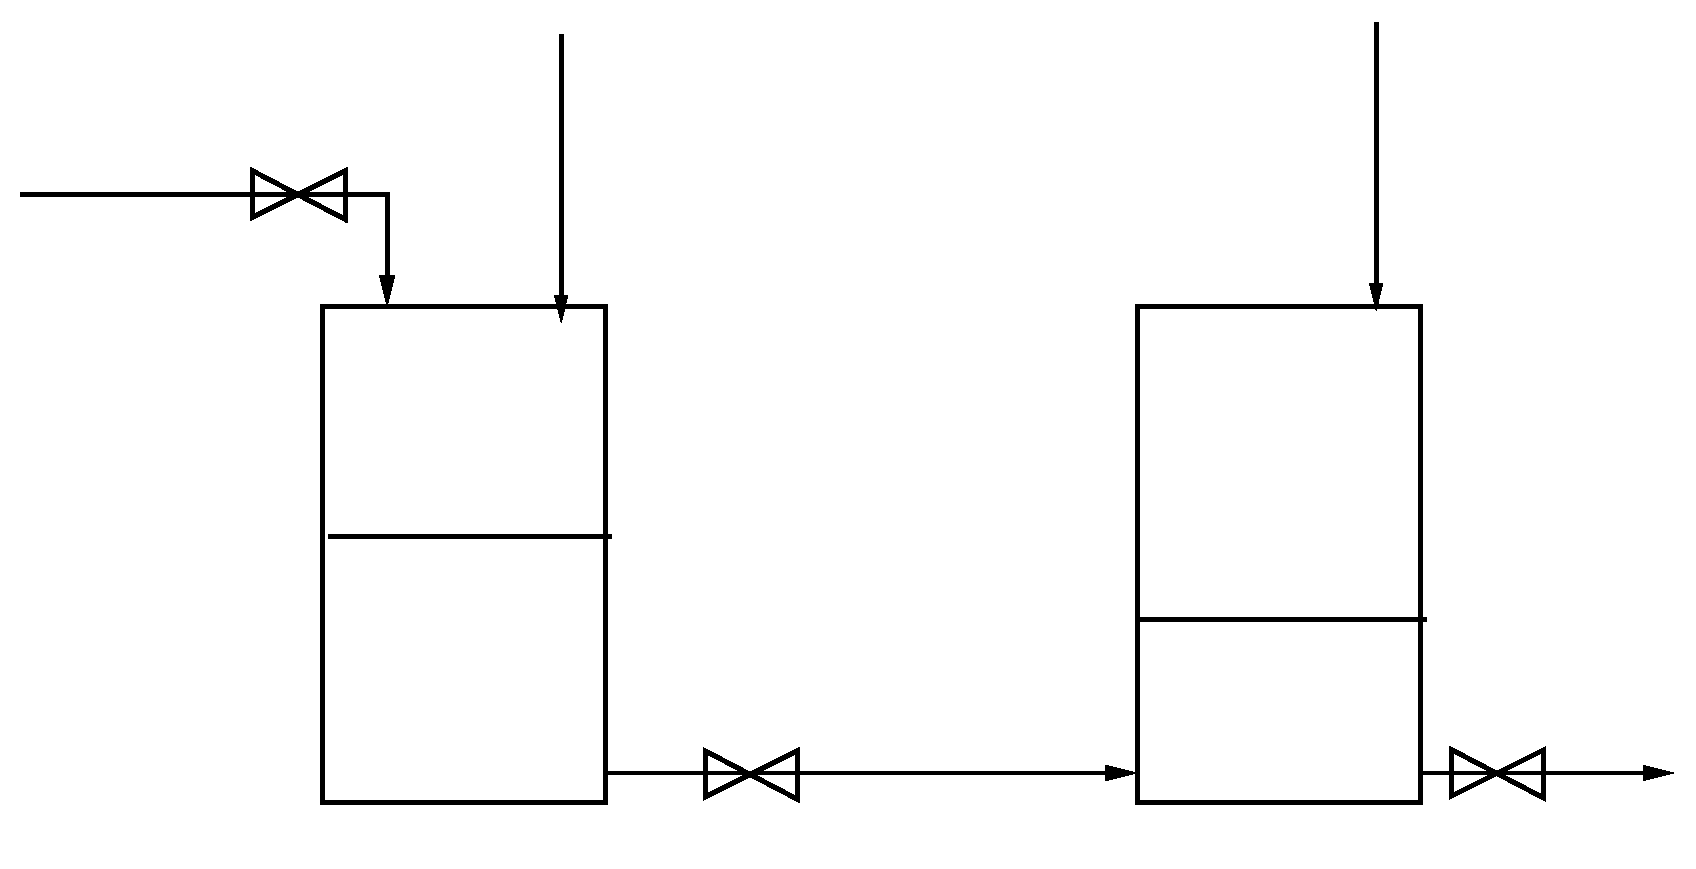
\includegraphics{two_tanks}%
\end{picture}%
\setlength{\unitlength}{4144sp}%
%
\begingroup\makeatletter\ifx\SetFigFont\undefined%
\gdef\SetFigFont#1#2#3#4#5{%
  \reset@font\fontsize{#1}{#2pt}%
  \fontfamily{#3}\fontseries{#4}\fontshape{#5}%
  \selectfont}%
\fi\endgroup%
\begin{picture}(12666,6356)(688,-5390)
\put(11881,-5326){\makebox(0,0)[lb]{\smash{{\SetFigFont{20}{24.0}{\rmdefault}{\mddefault}{\updefault}{\color[rgb]{0,0,0}$u_{22}$}%
}}}}
\put(1216,-646){\makebox(0,0)[lb]{\smash{{\SetFigFont{20}{24.0}{\rmdefault}{\mddefault}{\updefault}{\color[rgb]{0,0,0}$u_{11}$}%
}}}}
\put(9991,-4471){\makebox(0,0)[lb]{\smash{{\SetFigFont{20}{24.0}{\rmdefault}{\mddefault}{\updefault}{\color[rgb]{0,0,0}$x_2$}%
}}}}
\put(3871,-4021){\makebox(0,0)[lb]{\smash{{\SetFigFont{20}{24.0}{\rmdefault}{\mddefault}{\updefault}{\color[rgb]{0,0,0}$x_1$}%
}}}}
\put(6886,-5101){\makebox(0,0)[lb]{\smash{{\SetFigFont{20}{24.0}{\rmdefault}{\mddefault}{\updefault}{\color[rgb]{0,0,0}$u_{12}$}%
}}}}
\put(5041,-1006){\makebox(0,0)[lb]{\smash{{\SetFigFont{20}{24.0}{\rmdefault}{\mddefault}{\updefault}{\color[rgb]{0,0,0}$w_1$}%
}}}}
\put(11251,-1096){\makebox(0,0)[lb]{\smash{{\SetFigFont{20}{24.0}{\rmdefault}{\mddefault}{\updefault}{\color[rgb]{0,0,0}$w_2$}%
}}}}
\end{picture}%
}
\caption{Two tank system}
\label{fig:two_tanks}
\end{figure*}

We assume that the nominal value of $w_{1,n} = 0.1$ and that of $w_{2,n} =
5$. The set $\mathbb{W}$ is given by $\mathbb{W} := \set{w \mid 0\leq
  w_1\leq 0.2, 0 \leq w_2 \leq 10}$.

The input constraints are given by $\mathbb{U}_1 = \set {u_1 \mid 0
  \leq u_{11} \leq 10, 0 \leq u_{12} \leq 10}$ and $\mathbb{U}_2 =
\set{u_2 \mid 0 \leq u_{22} \leq 20}$.

Note that since we have a system of integrators, any level in the tank
can be stabilized as long as all the flows in the system are
balanced. Therefore, we choose the steady state in the tank as $x_s =
(20,20)$ (the level in both tanks are 20). The input steady state is
obtained by solving the following optimization problem
\[ min_{u}{u'Ru} \qquad \text{s.t~} Bu = -w_n ; u \in \mathbb{U} \]
in which $w_n$ is the nominal disturbance. For the choice of $R = I$
($I$ denotes the identity matrix), the input steady-state is obtained
as $u_s = (3.2667,3.3667,8.3667)$. 

The stage cost was chosen as $\ell(x,u) = 0.1 x'x + u'u$. We solve the
MPC problem in deviation variables, so that regulation to the origin
implies regulation to the steady state mentioned above. Following
the design procedure outlined in the previous sections, we chose 
(i) $V_f(x) = x'Px,\kappa_f(x) = Kx$ as the solution to the Riccatti
equation, 
(ii)$a$ = 1 and the terminal region as $x'Px \leq 1$. The choice of
  $a=1$ satisfies the requirements in Assumption \ref{ass:bsa}, (iii)
$\bar{V} = 100$, (iv) a prediction horizon of $N=15$ and (v)the controller that corrects for the error between the nominal
  and actual states was also chosen as $K(x-z)$ in which $K = \kappa_f(x)$.

For these choice of parameters, we followed the algorithm mentioned in
\citet{rakovic:kerrigan:kouramas:mayne:2003} to find the set
$\mathbb{V}$ (we chose $N=200$ and $\alpha = 1e-6$). Note that, since the original input set contained no
coupled inputs, the tightened set also contains no coupled inputs. 

In Figure \ref{fig:CL1}, we show the closed-loop response 
nominal closed-loop response of the level in the second tank and the for cooperative MPC rejecting a
persistent disturbance $w_k \in \mathbb{W}$.  We also show the cost-function $V_N(z,\tilde{\mathbf{v}})$ and
$V_N(x,\tilde{\mathbf{v}})$ to show that although the warm-start was
infeasible for the actual state, it was still feasible for the nominal
state and hence we could obtain the closed-loop guarantees for robust
cooperative MPC. Note that, for this particular disturbance
realization, we could not reset the nominal state to the actual state.

\begin{figure*}
\centering
\scriptsize
\resizebox{1\textwidth}{!}{\input{CL1}}
\caption{(Left) Closed-loop response (Right) Warm start rendered
  infeasible for actual state because of disturbance}
\label{fig:CL1}
\end{figure*}


In Figure \ref{fig:CL2}, we show the closed-loop response using a
modified version of Algorithm \ref{alg:rcoop}. The modification we
made are to reset the nominal state to the actual state at time $k$ if the
following conditions are satisfied (i)The nominal state $z(k)$ is inside $\mathbb{Z}_f$.
(ii) The warm start $\tilde{\mathbf{v}}(k)$ is feasible for the
actual state $x(k)$ and , (iii) The time elapsed since the last reset
is greater than $\bar{T}$
time periods (we chose $\bar{T} = 10$)

\begin{figure*}
\centering
\scriptsize
\resizebox{1\textwidth}{!}{% GNUPLOT: LaTeX picture with Postscript
\begingroup
  \makeatletter
  \providecommand\color[2][]{%
    \GenericError{(gnuplot) \space\space\space\@spaces}{%
      Package color not loaded in conjunction with
      terminal option `colourtext'%
    }{See the gnuplot documentation for explanation.%
    }{Either use 'blacktext' in gnuplot or load the package
      color.sty in LaTeX.}%
    \renewcommand\color[2][]{}%
  }%
  \providecommand\includegraphics[2][]{%
    \GenericError{(gnuplot) \space\space\space\@spaces}{%
      Package graphicx or graphics not loaded%
    }{See the gnuplot documentation for explanation.%
    }{The gnuplot epslatex terminal needs graphicx.sty or graphics.sty.}%
    \renewcommand\includegraphics[2][]{}%
  }%
  \providecommand\rotatebox[2]{#2}%
  \@ifundefined{ifGPcolor}{%
    \newif\ifGPcolor
    \GPcolortrue
  }{}%
  \@ifundefined{ifGPblacktext}{%
    \newif\ifGPblacktext
    \GPblacktexttrue
  }{}%
  % define a \g@addto@macro without @ in the name:
  \let\gplgaddtomacro\g@addto@macro
  % define empty templates for all commands taking text:
  \gdef\gplbacktext{}%
  \gdef\gplfronttext{}%
  \makeatother
  \ifGPblacktext
    % no textcolor at all
    \def\colorrgb#1{}%
    \def\colorgray#1{}%
  \else
    % gray or color?
    \ifGPcolor
      \def\colorrgb#1{\color[rgb]{#1}}%
      \def\colorgray#1{\color[gray]{#1}}%
      \expandafter\def\csname LTw\endcsname{\color{white}}%
      \expandafter\def\csname LTb\endcsname{\color{black}}%
      \expandafter\def\csname LTa\endcsname{\color{black}}%
      \expandafter\def\csname LT0\endcsname{\color[rgb]{1,0,0}}%
      \expandafter\def\csname LT1\endcsname{\color[rgb]{0,1,0}}%
      \expandafter\def\csname LT2\endcsname{\color[rgb]{0,0,1}}%
      \expandafter\def\csname LT3\endcsname{\color[rgb]{1,0,1}}%
      \expandafter\def\csname LT4\endcsname{\color[rgb]{0,1,1}}%
      \expandafter\def\csname LT5\endcsname{\color[rgb]{1,1,0}}%
      \expandafter\def\csname LT6\endcsname{\color[rgb]{0,0,0}}%
      \expandafter\def\csname LT7\endcsname{\color[rgb]{1,0.3,0}}%
      \expandafter\def\csname LT8\endcsname{\color[rgb]{0.5,0.5,0.5}}%
    \else
      % gray
      \def\colorrgb#1{\color{black}}%
      \def\colorgray#1{\color[gray]{#1}}%
      \expandafter\def\csname LTw\endcsname{\color{white}}%
      \expandafter\def\csname LTb\endcsname{\color{black}}%
      \expandafter\def\csname LTa\endcsname{\color{black}}%
      \expandafter\def\csname LT0\endcsname{\color{black}}%
      \expandafter\def\csname LT1\endcsname{\color{black}}%
      \expandafter\def\csname LT2\endcsname{\color{black}}%
      \expandafter\def\csname LT3\endcsname{\color{black}}%
      \expandafter\def\csname LT4\endcsname{\color{black}}%
      \expandafter\def\csname LT5\endcsname{\color{black}}%
      \expandafter\def\csname LT6\endcsname{\color{black}}%
      \expandafter\def\csname LT7\endcsname{\color{black}}%
      \expandafter\def\csname LT8\endcsname{\color{black}}%
    \fi
  \fi
  \setlength{\unitlength}{0.0500bp}%
  \begin{picture}(7200.00,3024.00)%
    \gplgaddtomacro\gplbacktext{%
      \csname LTb\endcsname%
      \put(814,704){\makebox(0,0)[r]{\strut{} 10}}%
      \put(814,1732){\makebox(0,0)[r]{\strut{} 20}}%
      \put(814,2759){\makebox(0,0)[r]{\strut{} 30}}%
      \put(946,484){\makebox(0,0){\strut{} 0}}%
      \put(1433,484){\makebox(0,0){\strut{} 10}}%
      \put(1921,484){\makebox(0,0){\strut{} 20}}%
      \put(2408,484){\makebox(0,0){\strut{} 30}}%
      \put(2896,484){\makebox(0,0){\strut{} 40}}%
      \put(3383,484){\makebox(0,0){\strut{} 50}}%
      \put(176,1731){\rotatebox{-270}{\makebox(0,0){\strut{}Level in Tank-1}}}%
      \put(2164,154){\makebox(0,0){\strut{}Time}}%
      \put(1921,1218){\makebox(0,0)[l]{\strut{}$S_K(\infty)$ bound}}%
    }%
    \gplgaddtomacro\gplfronttext{%
      \csname LTb\endcsname%
      \put(2396,2586){\makebox(0,0)[r]{\strut{}Actual}}%
      \csname LTb\endcsname%
      \put(2396,2366){\makebox(0,0)[r]{\strut{}Nominal}}%
    }%
    \gplgaddtomacro\gplbacktext{%
      \csname LTb\endcsname%
      \put(4109,484){\makebox(0,0){\strut{} 0}}%
      \put(4517,484){\makebox(0,0){\strut{} 2}}%
      \put(4925,484){\makebox(0,0){\strut{} 4}}%
      \put(5334,484){\makebox(0,0){\strut{} 6}}%
      \put(5742,484){\makebox(0,0){\strut{} 8}}%
      \put(6150,484){\makebox(0,0){\strut{} 10}}%
      \put(6282,704){\makebox(0,0)[l]{\strut{} 0}}%
      \put(6282,1115){\makebox(0,0)[l]{\strut{} 100}}%
      \put(6282,1526){\makebox(0,0)[l]{\strut{} 200}}%
      \put(6282,1937){\makebox(0,0)[l]{\strut{} 300}}%
      \put(6282,2348){\makebox(0,0)[l]{\strut{} 400}}%
      \put(6282,2759){\makebox(0,0)[l]{\strut{} 500}}%
      \put(7051,1731){\rotatebox{-270}{\makebox(0,0){\strut{}Cost}}}%
      \put(5129,154){\makebox(0,0){\strut{}Time}}%
    }%
    \gplgaddtomacro\gplfronttext{%
      \csname LTb\endcsname%
      \put(5163,2586){\makebox(0,0)[r]{\strut{}$V_N^\beta(x,\tilde{\mathbf{v}})$}}%
      \csname LTb\endcsname%
      \put(5163,2366){\makebox(0,0)[r]{\strut{}$V_N^\beta(z,\tilde{\mathbf{v}})$}}%
      \csname LTb\endcsname%
      \put(5163,2146){\makebox(0,0)[r]{\strut{}$\bar{V}$}}%
    }%
    \gplbacktext
    \put(0,0){\includegraphics{mpc/CL2}}%
    \gplfronttext
  \end{picture}%
\endgroup
}
\caption{(Left) Closed-loop response. Notice that we reset the state
  around t = 15 (Right) Warm start rendered
  infeasible for actual state because of disturbance}
\label{fig:CL2}
\end{figure*}



\section{Related Work}
\label{sec:related}
Cooperative MPC has evolved as a attractive architecture for
distributed control because it solves the centralized control
problem, and inherits the desirable closed-loop properties of
centralized control. 
In the previous sections, we described
cooperative MPC based on the ``primal decomposition'' of the
centralized optimization
problem. In the primal decomposition, the centralized optimization
problem is solved directly using parallel optimization
architectures. \citet{liu:chen:pena:christofides:2010} also use the
primal decomposition to solve the centralized optimization problem for a
non-linear process model. They use a closed-form controller $u=h(x)$
for which a Lyapunov function is known as a reference controller to
design their MPC optimization problem. Thus, they ensure that the MPC
inherits the stability properties of $u=h(x)$. Note that $u=h(x)$ also
provides a warm start, even when the actual and predicted states are
different. However, since this stability constraint is a coupled
constraint, there can be no guarantees about the convergence of the
parallel optimization routine. The authors propose both a Jordan
algorithm (all subsystems optimize in parallel) and a Gauss-Siedel
algorithm (subsystems optimize in sequence). In comparison, in
\citet{stewart:wright:rawlings:2011}, the authors propose a Jordan
algorithm for non-linear MPC that converges to the centralized optimal
solution. Since, for non-convex problems, the Jordan optimizations
does not necessarily produce a descent direction, the authors propose
a sequential procedure to obtain a descent direction using the
solutions obtained from each subsystem. This overhead is not
equivalent to implementing a coordinator as each subsystem only
calculates an objective function in the second phase of the algorithm
in which a descent direction is
determined. \citet{maestre:pena:camacho:alamo:2011} propose a primal
decomposition approach to cooperative MPC based on agent
negotiation. The advantage of their procedure is that agents need only
know models of the subsystems whose inputs affect their states. In the
proposed method, each agent optimizes its local objective over all
the inputs that affect its dynamics, and share the proposed solution
with other agents. The other agents evaluate the proposal for
cost-drop and constraint violation and communicate back to the
original agent making the proposal, who can then decide to accept or
reject the proposal. The authors ensure that only feasible proposals
are accepted. The drawback of the proposed architecture, however, is
that (i) the agents have to solve larger optimization problems
(because they have to optimize over all the inputs that affect their
state), and (ii) the convergence to the centralized optimal solution
cannot be guaranteed. Stability is guaranteed using the warm
start. \citet{maestre:pena:camacho:2011} use game-theoretic analysis
to propose a distributed optimization framework. In this method, each
node, optimizes its local objective over its local decisions while
keeping the other subsystem decisions fixed. After completion of the
optimizations, the agents compute their local objectives for all
possible combinations of the overall system input (based on optimized
solution of the agents and the warm start). Upon sharing the
objectives, the agents then select the input that minimizes the
overall cost. Thus, each agent cooperatively makes a decision. However,
the proposed algorithm also fails to establish convergence to the
centralized optimal on iteration. Stability is guaranteed by design of
terminal region and warm-start. \citet{muller:revle:allgower:2012}
propose a optimization algorithm based on each node optimizing over
its local optimization problem. They use a terminal region which is a
sub-level set of the terminal penalty. Because of the presence of
coupled constraints, input directions are discarded if they are not
feasible, based on a check made after the optimizations. To ensure
cost-drop, the centralized objectives are also evaluated after the
optimizations and inputs that do not achieve cost-drop are
discarded. The model considered by the authors had coupling introduced
only via the constraints (both in the objective function and the
constraints). The authors also provide a method to define local time
varying terminal regions, so that the coupled terminal region
constraint is satisfied if each subsystem satisfies its local time
varying terminal region constraint. The algorithm provided by the
authors, satisfies the requirements of the optimizer for suboptimal
MPC, but again, does not give any convergence guarantees. The
requirement of decoupled dynamics is important in problems like multi
vehicle synchronization
etc. \citet{johansson:speranzon:johansson:johansson:2006} use a primal
decomposition to solve a multi-vehicle consensus problem as a MPC
problem. While the dynamics are decoupled, the consensus point,
similar to terminal equality constraint, is the complicating
constraint. Unlike the MPC problems where the objectives are also
constrained because of the dynamics, the multi-vehicle receding
horizon problem falls into the category of uncoupled objective but
coupled constraints. The author's use a primal decomposition which
generates feasible iterate that reduce the objective function
value. However, in order to ensure that the centralized optimal
solution is achieved, the authors use a coordinator, which is based on
sub-gradient optimization to handle the coupled constraint. It is
interesting to note that economic MPC problems for plants with linear
economics and dynamics also have the characteristic that the
objectives are separable and the constraints are coupled.

A common theme in optimizing the centralized  problem is
that it is not easy to guarantee convergence to the optimal
solution. However, stability can be guaranteed because every iterate
is designed so that it reduces the cost while remaining feasible. In
contrast, there are a lot of cooperative MPC algorithms which are
based on the ``dual decomposition''. In the dual decomposition, the
coupled constraints are relaxed by using the Lagrangian of the
objective function. For a fixed value of the Lagrange multipliers
(also called as prices or dual variables), the relaxed problem can be solved using
parallel optimization methods as there are no complicating
constraints. Upon achieving the solution to the relaxed problem, the
Lagrange multipliers are updated. The Lagrange multiplier update is
usually done by a coordinator. These algorithms often converge faster
to the optimal solution. However, their main disadvantage is that they
are guaranteed to produce a feasible iterate only upon
convergence. Since stability theory for suboptimal MPC rely on the
fact that the suboptimal iterate is feasible, cooperative MPC
algorithms using dual decmposition use stability theory based on
optimal MPC to ensure stability. Therefore, a common theme in dual
decomposition based cooperative MPC algorithms are a coordinator layer
and a requirement that the iterates converge. 

The cooperative MPC algorithms using dual decomposition differ based on
the technique used to update the dual variables. In
\citet{cheng:forbes:yip:2007}, the dual variables (prices) are updated
using a sub-gradient based optimization algorithm. Subgradient methods
are also used in \citet{ma:anderson:borrelli:2011},
\citet{wakasa:arakawa:tanka:akashi:2008},
\citet{marcos:forbes:guay:2009}. \citet{morocan:bourdais:dumur:buisson:2011}
formulate the building control problem as a MPC problem with linear
objectives and use Benders decomposition to solve the problem. Benders
decomposition is a widely popular parallel algorithm when by fixing the
value of a complicating variable, the remaining problem can be
completely separated. \citet{scheu:marquardt:2011} propose a dual
decomposition algorithm without a coordination layer. They augment the
local subsystem objective function with the sensitivity of the
objectives and constraints of other subsystems to obtain updates for
the dual variables along with the primal variables. However, this
method generates a feasible solution only upon
convergence. \citet{giselsson:doan:keviczky:schutter:rantzer:2012}, \citet{giselsson:rantzer:2010}
propose a dual decomposition algorithm with a stopping criteria based
on the objective value to ensure stability. They advocate the use of
long prediction horizon along with results obtained in
\citet{grune:2009} to determine bounds on the value of the objective
function so that stability can be
guaranteed. \citet{doan:keviczky:necoara:diehl:schutter:2009} modified
the Han's algorithm which is a dual decomposition based algorithm for
the special structure of the MPC problem. Although the method uses
communication between directly connected subsystems, stability is
guaranteed only upon convergence. \citet{necoara:doan:suykens:2008}
use a smoothing technique to simplify the dual problem. With the
smoothing technique, the coordinator problem for finding the Lagrange
multiplier updates becomes easier. The algorithm also gives bounds on
the number of iterations so that the optimal solution and constraint
violation are within a pre-specified limit ($\epsilon$ approximation of
the centralized problem). The main advantage is that the dual
decomposition based on proximal center is order of magnitude faster
than other sub-gradient based methods. Finally,
\citet{doan:keviczky:schutter:2011}, propose a primal feasible dual
gradient approach, that generates a primal feasible solution  that
achieves cost-drop in a
finite number of iterations based on an averaging scheme of the primal
variables at each iteration. 

\citet{christofides:scattolini:pena:liu:2012} is a recent review of different algorithms for distributed
MPC. \citet{necoara:nedelcu:dumitrache:2011} provides an excellent overview of the different
optimization problems and parallel solution strategies that are seen
in control and estimation.

\citet{trodden:richards:2006,trodden:richards:2007} propose a tube based robust distributed
MPC algorithm. In their method, at each sampling time, only one
subsystem performs optimization. The subsystem optimizes only over its
decision variables, keeping all other subsystem decisions fixed from
the previous iteration. This method is also an example of primal
decomposition. \citet{richards:how:2004} present a robust tube-based
MPC for systems with decoupled dynamics. The coupling constraints are
coupled output constraints. Their algorithm is based on the
Gauss-Siedel iterations.



\section{Conclusions}
\label{sec:conclusions}

{\em{placeholder for now...will write it soon}}
We propose a cooperative MPC algorithm in which each agent solves the
centralized optimization problem subject to its own inputs. The
algorithm uses a primal decomposition to solve the centralized problem
using a Jordan algorithm. Stability is ensured by designing
appropriate terminal region and penalties and using suboptimal theory.
To ensure that the Jordan algorithm converges to the optimal solution, we described two techniques to
remove coupled constraints that are required to ensure stability from the centralized MPC optimization
problem. With the relaxed optimization problems, we can ensure that
cooperative MPC has stability as well as performance
guarantee. Finally, we used techniques from MPC using tubes to propose
a robust cooperative MPC controller that has both stability and
performance guarantees.


\bibliographystyle{abbrvnat}
{\bibliography{abbreviations,articles,proceedings,books,unpub}
}
\end{document}











